\documentclass[../manuscript.tex]{subfiles}
\def\biblio{\bibliographystyle{plainnat}\bibliography{bibliography}}

\usepackage{Sweave}
\begin{document}
\section[Experiment 1]{Experiment 1. Scaling of critical spacing with eccentricity.}\label{sec:constant}

\subsection{Methods}

We presented stimuli at eccentricities of 10, 6.67, 4.44, and 2.96
degrees, using the parameters described above for Movie 1
but scaling all spatial parameters (${\Delta}x$, $w$, $1/f$) of the
elements along with the eccentricity; i.e. at eccentricity of 6.67
degree, ${\Delta}x$ and $w$ decreased to 2/3 the value used at 10
degrees and $f$ increased to 3/2 its value. The global apparent motion
was shown over 4 stations at intervals of ${\Delta}t=100$ ms.

At each eccentricity, we varied the number of elements in the circle (and consequently the inter-element spacing) in the circle using the method of constant stimuli, using
values chosen for each subject based on preliminary sessions.

\subsection{Results}

\begin{figure}
	\begin{subfigure}[b]{.3\linewidth}
			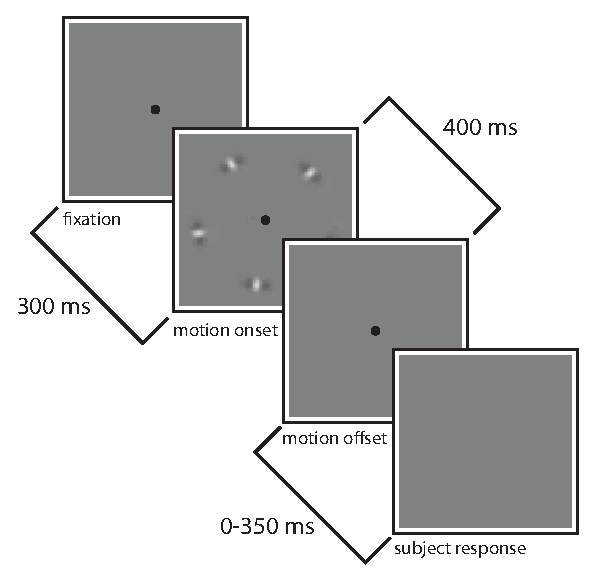
\includegraphics[width=\linewidth]{A}	
			\subcaption{Task illustration. Subjects first fixate and after a brief delay a motion stimulus of constant duration appears. Subjects judge the apparent direction of motion and respond by turning a knob before the time window has expired. Subject receives feedback about whether their response falls inside the time window.}
			\label{fig:task}
	\end{subfigure}	
	\begin{subfigure}[b]{.6\linewidth}
		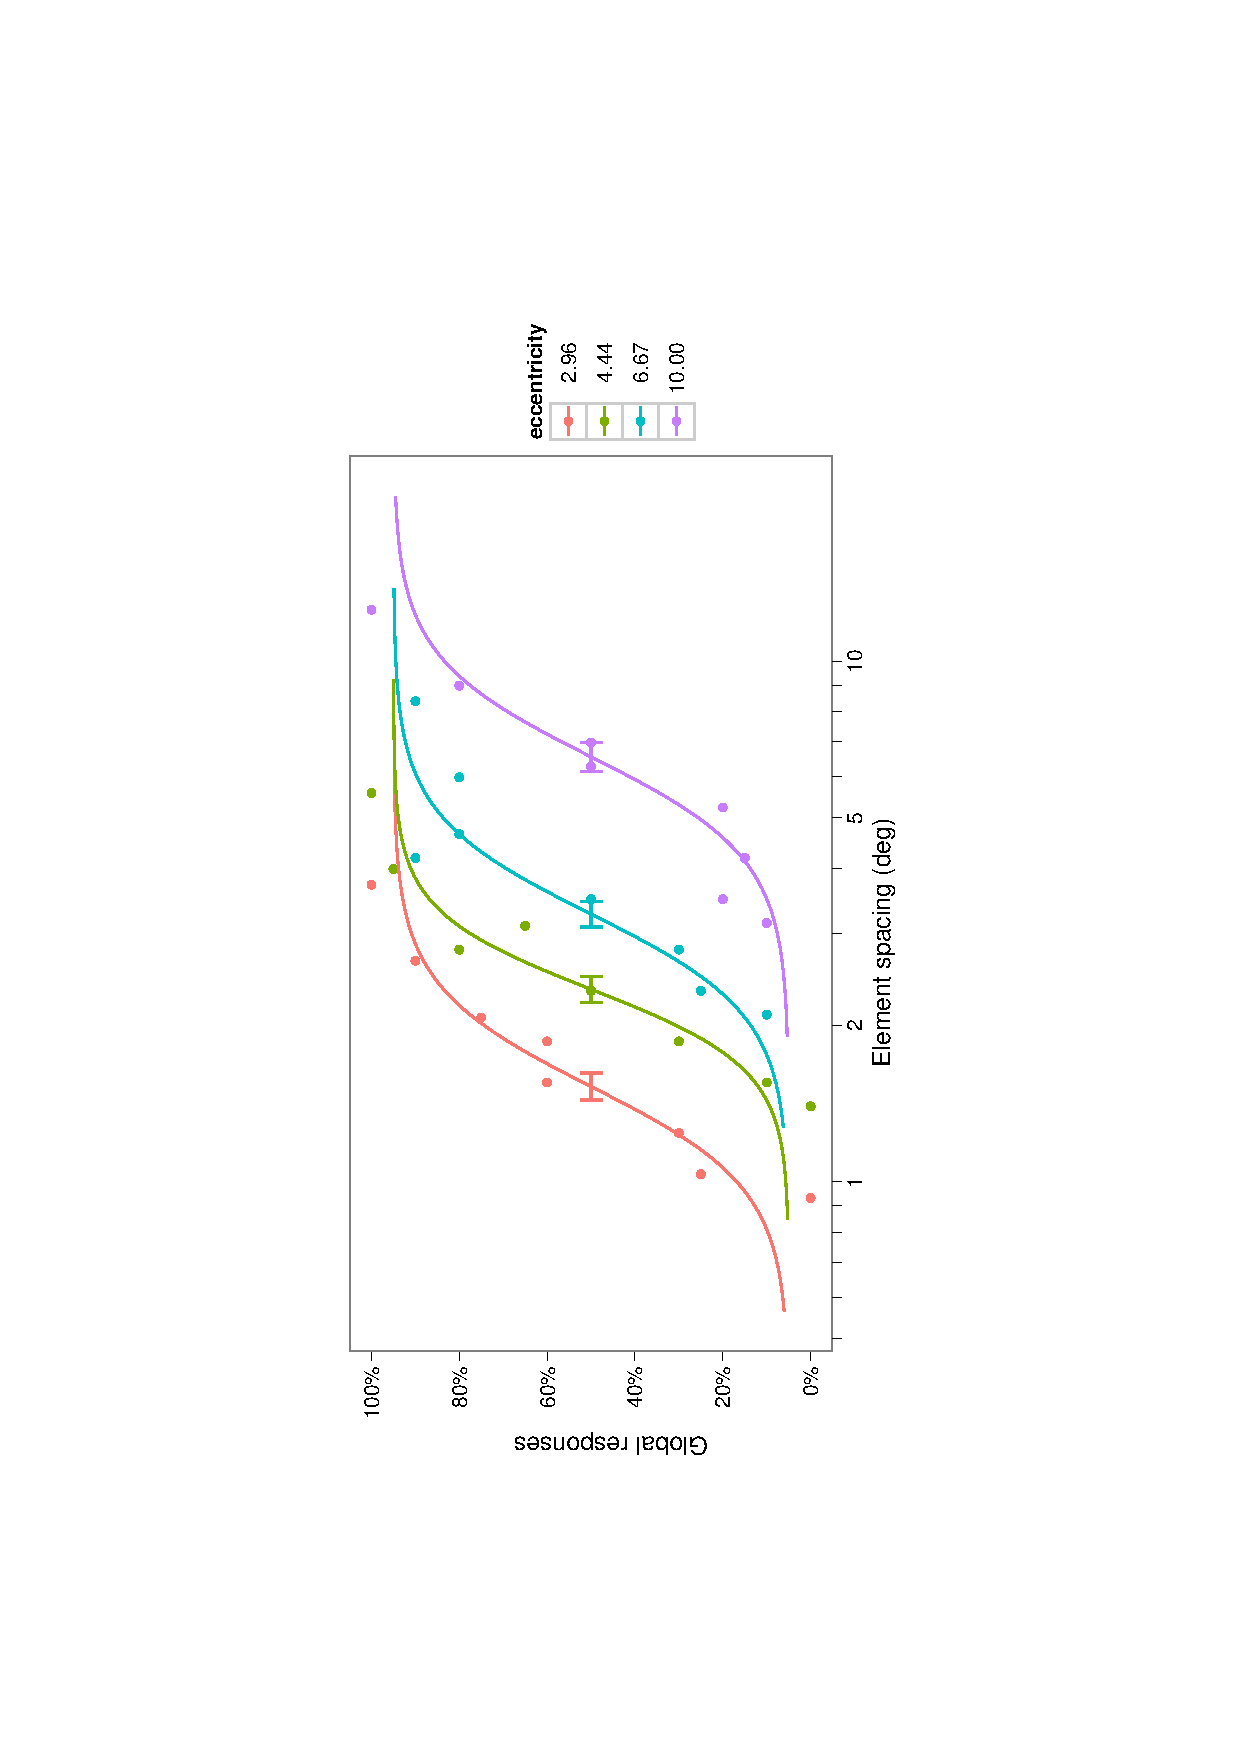
\includegraphics[angle=270, width=\linewidth]{c}	
		\subcaption{Example data. The responses of observer DT to incongruent stimuli are plotted as a function of between-element spacing, for four values of eccentricity. The values plotted are the proportion of responses that agree with the global motion direction.  Curved lines are fit to the data by a cumulative logistic with a constant guess rate. The point of subjective equality (PSE) is indicated on each fit.}
		\label{fig:sigmoids}
	\end{subfigure}
	\begin{subfigure}[b]{.3\linewidth}
		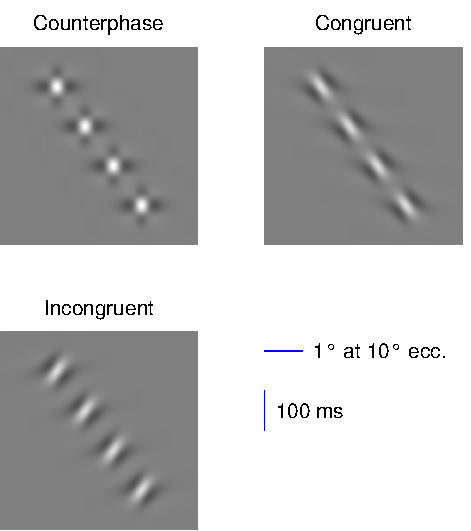
\includegraphics[width=\linewidth]{B}	
		\subcaption{Example stimuli in space-time form, where time progresses down along the vertical axis. Stimuli were `congruent', 'conterphase' or incongruent, based on whether the global direction of motion agreed with the local. Counterphase stimuli are a superposition of congruent and incongruent stimuli.}
		\label{fig:stimuli}
	\end{subfigure}
	\begin{subfigure}[b]{.6\linewidth}
		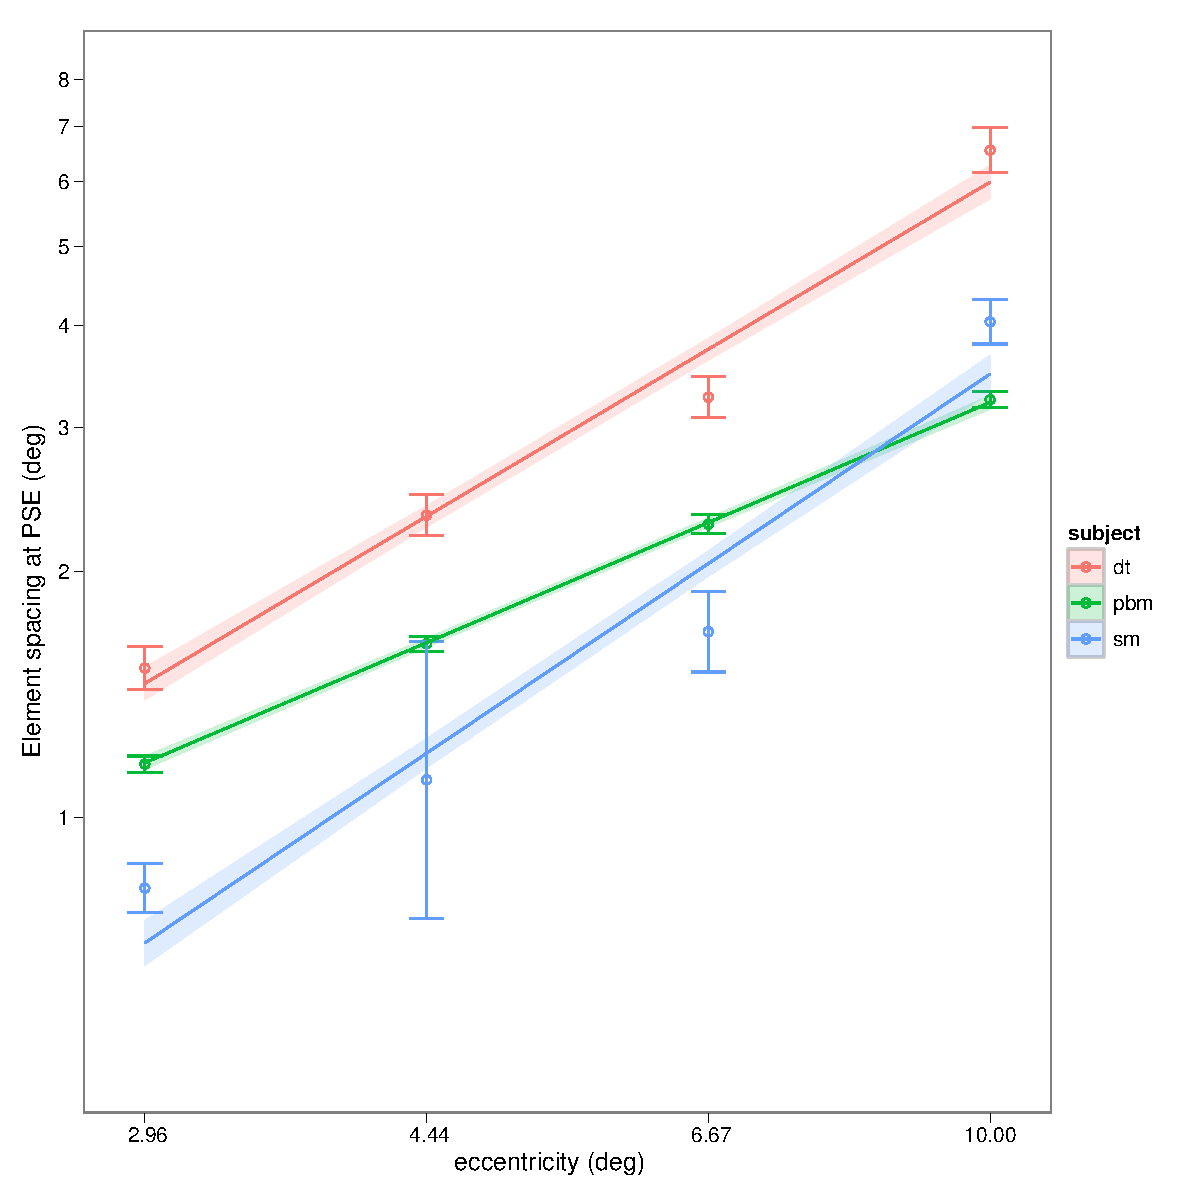
\includegraphics[width=\linewidth]{d}
		\subcaption{Points of subjective equality (target separation subserving 50\% response probability) for each eccentricity for all subjects. Intervals show standard errors. Lines show a power-law fit between eccentricity and critical target separation. Shaded region shows standard error of the power-law fit.}
		\label{fig:scaling}
	\end{subfigure}
        \caption{}
        \label{fig:constant}
\end{figure}

\todo{The sigmoids need to be refit with a constant slope (since that is how we will approach the variations and occlusions data; QUEST data doesn't well support calculating slope and it adds noise to the PSE calculation. Also, look at different choices of scaling in element spacing to see what is the best fit? Maybe plot on log but fit linearly? Does that scale?}

Using the third of trials where global motion opposed local, we obtained a
psychometric function relating the target spacing to the probability
that the stimulus is seen to rotate in the direction of the global
motion. The data were fit to a cumulative logistic function using a
maximum likelihood estimator. We found the spacing where the
logistic curve intersected 50\%.

We fit the subject's responses at each eccentricity to a logistic function, as illustrated for subject D.T. by the curves in \autoref{fig:sigmoids}. A separate curve was fit for each eccentricity, with a guessing rate that was fit for each subject \citep{Wichmann:2001kx} \todo{actually do this}. From these fits we estimated the point at which subject responses would be equally split between local and global directions of motion. This point of subjective equivalence (PSE) \todo{I'm not happy abut calling this 'subjective equivalence' because I'm not sure what the stimuli are 'equivalent' to, they're not metamers. Perhaps a point of equivocation?} is indicated by the horizontal error bars in \autoref{fig:sigmoids}, and are plotted using vertical error bars in \autoref{fig:scaling} for all subjects. This spacing at the PSE appears to scale with the eccentricity of the stimulus. We made another fit to a model where the size of the PSE was proportional to the stimulus eccentricity; this model fit is shown as lines and shaded regions in \autoref{fig:scaling}. When compared to estimates taken at each individual eccentricity, we saw XXXX significant differences at YYYY conditions. \todo{OK, so what's the appropriate test? Fit a model plus one data point, at each data point, and see if the added coefficient was a significant change? (ONLY X conditions, significant marked with a star; were these differences explainable?)}

The scalar dependence on critical separation is broadly similar to the phenomenon of crowding, in which recognition or discrimination of a target object is impaired by the presence of flanking objects. \todo{does this need a cite? ``Who defined crowding'' is a hard thing to cite.} It is also suggestive of a cortical mechanism. There are several areas of cortex that are organized into retinotopic maps\todo{cite?}. The foveated scaling of space within these maps has the property that network interactions that span a constant distance in cortex, including V1, will correspond to interactions in visual space whose distance approximately scales with retinal eccentricity. \todo{I can cite papers for MT and V4 that make the claim that those maps are just simple linear scalings of the V1 map.}

\biblio
\end{document}
